\documentclass[12pt]{article}
\usepackage{amsmath, amssymb, graphicx, hyperref}
\usepackage{geometry}
\usepackage{amsmath, amssymb, amsthm}
\usepackage{algorithm}
\usepackage{algorithmic}
\usepackage{float}
\usepackage{fancyhdr}
\usepackage{array}
\usepackage{longtable}
\usepackage{geometry}
\usepackage{listings}
\usepackage{tikz}
\usepackage{tcolorbox}
\usetikzlibrary{matrix}
\usepackage{url}
\usepackage{xcolor}

\lstset{
    basicstyle=\ttfamily\footnotesize,
    breaklines=true,
    frame=single,
    rulecolor=\color{black},
    keywordstyle=\color{blue},
    stringstyle=\color{teal},
}
\geometry{a4paper, margin=1in}
\pagestyle{fancy}

%\usepackage[margin=1in]{geometry}
\begin{document}

\begin{titlepage}                                             
\pagestyle{empty}                                             
\centering                                                   

\includegraphics[width=0.7\textwidth]{IITH.png} \\ 
\vspace{60mm}                                                 
\hrule\vspace{5mm}                                           
{\LARGE \textbf{{EIGENVALUE CALCULATION}}} \\          
\vspace{5mm}\hrule\vspace{20mm}                        
{\large Arjun Pavanje} \\ \vspace{2mm}                           
{\large (EE24BTECH11005)}                        
\vfill                                                       
{\small IIT Hyderabad\\ \today}               
\cleardoublepage                                            
\end{titlepage}

\section{Introduction}


Eigenvalue computation is a cornerstone of numerical linear algebra with widespread applications across sciences and engineering. This report delves into the implementation of eigenvalue computation using Householder transformations and Givens rotations. 
\section{Definition}
Firstly, what are eigenvalues? Eigenvalues of a matrix $A$ are those values $'\lambda'$ that satisfy the relation $A\mathbf{v}=\lambda\mathbf{v}$.\\\\
It is important to understand the intuitive sense behind them. The $A\mathbf{v}$ represents a linear transformation (rotation/scaling/shear/translation) being applied on $\mathbf{v}$. $\lambda\mathbf{v}$ represents the vector $\mathbf{v}$ being scaled by a factor of $\lambda$. Both of them being equal implies that for a matrix $A$, there exist some special vectors $\mathbf{v}$ for which applying the linear transformation represented by the matrix just has a scaling effect on it, i.e. $\mathbf{v}$ lies in its own span after going through the linear transformation represented by $A\mathbf{v}$.\\\\

Now, to define it a little more rigorously,\\ 
\textit{Eigenvalues} are defined as scalars \( \lambda \in \mathbb{C} \) for which there exists a non-zero vector $( \mathbf{v} \in \mathbb{C}^n, v \ne 0)$ such that:
\begin{align*}
A \mathbf{v} = \lambda \mathbf{v}
\end{align*}
where $ A $ is an $(n \times n)$ matrix. The scalar $(\lambda)$ is the factor by which the vector $\mathbf{v}$, called the \textit{eigenvector}, is scaled under the linear transformation represented by \( A \).


\section{Applications}
Eigenvalue computation has widespread applications in various branches of science and engineering.

\section{Theory}

\subsection{Why Not Solve $\det(A - \lambda I) = 0 $ Directly?}
The characteristic polynomial $\det(A - \lambda I) = 0$ theoretically provides all eigenvalues of $A$. However, solving it directly is impractical for several reasons:
\begin{enumerate}
    \item \textbf{No closed form solution: } According to Abel-Ruffini theorem, there is no general solution for a polynomial of degree $n$ beyond $n$ greater than $4$. What it means is, like how there exists a general solution of a quadratic equation 
    \begin{align*}
    \frac{-b \pm \sqrt{b^2-4ac}}{2a}
    \end{align*}
    , similar formulae (but much more complicated) exist for cubic and biquadratic polynomials. But no such generalized formula to find all the roots exist for quintic polynomials and beyond.
    \item \textbf{Numerical instability:} The polynomial roots are highly sensitive to perturbations, leading to numerical instability.
    \item \textbf{Computational Expense:} For large matrices, the degree of the polynomial is high, making root-finding algorithms computationally expensive.
\end{enumerate}
\subsection{Schur Form}

The Schur form is a useful matrix decomposition where any square matrix $A \in \mathbb{C}^{n \times n}$ can be written as $ A = Q T Q^H $, where $Q$, is a unitary matrix and $T$ is an upper triangular matrix. The eigenvalues of $A$ are the diagonal elements of $T$, making the Schur form desirable for finding eigenvalues. It simplifies computations greatly. To find it, QR algorithm is implemented.

\subsection{QR Decomposition}

QR decomposition is a matrix decomposition technique where a given matrix $A$ is decomposed into a product of two matrices (one orthogonal, one upper triangular):
\begin{align*}
A = QR,
\end{align*}
where:
\begin{itemize}
    \item $Q$ is an orthogonal matrix, meaning $(Q^{\top} Q = I)$,
    \item $R$ is an upper triangular matrix.
\end{itemize}
QR decomposition is widely used in solving linear systems, eigenvalue problems, etc. This is due to numerical stability of QR algorithms as compared to others.
\subsection{Similar Matrices}
Two square matrices $A$ and $B$ of size $n \times n$ are said to be $similar$ if there exists an invertible matrix $P$ such that:
\begin{align*}
B = P^{-1} A P.
\end{align*}

\subsubsection{Properties of Similar Matrices:}
\begin{enumerate}
\item \textbf{Same Eigenvalues:} Similar matrices share the same eigenvalues, including their algebraic multiplicities.
\item \textbf{Determinant and Trace:} The determinant and trace of similar matrices are equal.
\item \textbf{Same Rank:} Similarity transformations do not change the rank of a matrix.
\end{enumerate}
\subsubsection{Intuition:}
Similarity captures the idea that $A$ and $B$ represent the same linear transformation but in different bases. The matrix $P$ provides the change of basis.
\subsubsection{Proof that Similar Matrices Have the Same Eigenvalues}
Given that $A$, $B$ are similar matrices, and $P$ is an invertible matrix such that $B=P^{-1}AP$
By definition of eigenvalues,
\begin{align*}
    \det(B-\lambda I)&=\det(P^{-1}AP -\lambda I)\\
    &=\det(P^{1}AP -\lambda P^{-1}P)\\
    &=\det(P^{-1})\det(A-\lambda I)\det(P)\\
    &=\det(P^{-1}P)\det(A- \lambda I)\\
    &=\det(A-\lambda I)
\end{align*}

\subsection{Eigenvalue preservation and Convergence}

The QR decomposition of a square matrix $A$ is the factorization:
\begin{align*}
A = Q R,
\end{align*}
where $Q$ is an orthogonal matrix $(Q^{\top} Q = I)$ and $R$ is an upper triangular matrix. The QR algorithm iteratively computes:
\begin{align*}
A_{k+1} = R_k Q_k,
\end{align*}
where $A_k = Q_k R_k$ is the QR decomposition of $A_k$. 
Eventually repeating this process will lead to the matrix $A_n$ being an upper triangular matrix, which is what we desire. When the matrix is upper triangular, we can just note its principal diagonal elements, as they will be the eigenvalues of the matrix.
\subsubsection{Eigenvalue Conservation}

To see why eigenvalues are conserved during the QR iteration, consider the similarity transformation performed at each step:
\begin{align*}
A_{k+1} = R_k Q_k = Q_k^{\top} A_k Q_k.
\end{align*}
Given, $A_k = Q_k R_k$ and $A_{k+1} = R_k Q_k$. Consider the definition of eigenvalue
\begin{align*}
\det(A_{k+1} - \lambda I) = \det(R_k Q_k - \lambda I).
\end{align*}
Writing $I$ as $Q_k^{\top} Q_k$ and $R_k$ as $Q_k^{\top}A_k$
\begin{align*}
    \det(R_k Q_k - \lambda I)&=\det(Q_k^{\top}A_k Q_k - \lambda Q_k^{\top} Q_k)\\
    &= \det(Q_k^{\top})\det(A_k -\lambda I)\det(Q_k)\\
    &= \det(Q_k^{\top} Q_k)\det(A_k -\lambda I)\det(Q_k)\\
    &= \det(A_k -\lambda I)\quad \quad \quad \quad (\because Q_k^{\top}Q_k = I)
\end{align*}
So, $A_{k+1}, A_k$ are similar, i.e. eigenvalues are conserved in the transformation of $A_k$ to $A_{k+1}$

\subsubsection{Convergence to Upper Triangular Form}
The QR iteration gradually reduces $A_k$ to an upper triangular form. When the matrix is upper triangular, we can just note its principal diagonal elements, as they will be the eigenvalues of the matrix. The eigenvalues of a matrix are conserved in the QR algorithm because the
process relies on similarity transformations. Successive iterations lead to con-
vergence towards an upper triangular form, with the eigenvalues appearing on
the diagonal. For faster convergence, shift strategies such as Rayleigh’s quotient
are employed, ensuring numerical stability and efficiency.

\subsection{Hessenberg Form via Householder Transformation}
A square matrix A of order $n \times n$ is said to be in upper Hessenberg form if all the entries below the first subdiagonal are zero. To define it a little more mathematically, if the elements of a matrix are represented as $[a_{ij}]$, it is said to be in Upper Hessenberg iff 
\begin{align*}
    a_{ij}=0,  \forall i>j+1
\end{align*}
For example:
\begin{align*}
H = \begin{bmatrix}
\times & \times & \times & \times \\
\times & \times & \times & \times \\
0 & \times & \times & \times \\
0 & 0 & \times & \times
\end{bmatrix}.
\end{align*}
Applying QR decomposition to reach Schur-form to the matrix after it is in Upper Hessenberg form greatly accelerates rate of convergence.\\
Householder transformations are used to reduce a general matrix $A$ to Hessenberg form. A Householder reflector is an orthogonal matrix defined as:
\begin{align*}
P = I - 2\textbf{uu}^{\top} \\
\end{align*}
where $\|\textbf{u}\|=1$\\
If the entries of the matrix are complex, transpose is to replaced with conjugate transpose.
Vector $\textbf{u}$ must be carefully chosen such that the resultant matrix $P$ obtained from it must zero out all elements below the first subdiagonal for that particular column while maintaining similarity to preserve eigenvalues.

\subsubsection{Choosing the Vector $\mathbf{u}$}

For a given column vector $x \in \mathbb{R}^n$, the vector $u$ is chosen as:
\begin{align*}
\mathbf{u} = \frac{\mathbf{x} - \|\mathbf{x}\| \rho \mathbf{e_1}}{\|\mathbf{x} - \|\mathbf{x}\| \rho \mathbf{e_1}\|}
\end{align*}
where:
\begin{itemize}
    \item $\mathbf{e_1}$ is impulse vector of appropriate dimensions, first element 1
    \item $\rho$ is something we have a degree of freedom in choosing as long as $|\rho|=1$
\end{itemize}
Usually, $\rho=-sign(x_1)$, but here for ease of calculation $\rho= -e^{j\phi}$ where $x_1=|x_1| e^{j\phi}$\\\\
We then construct Householder reflector matrix $P_1$ as,

\begin{align*}
P_1 = \begin{bmatrix}
1 & 0 & 0 & 0 & 0 & 0 \\
0 & \times & \times & \times & \times & \times \\
0 & \times & \times & \times & \times & \times \\
0 & \times & \times & \times & \times & \times \\
0 & \times & \times & \times & \times & \times \\
0 & \times & \times & \times & \times & \times \\
\end{bmatrix} =
\begin{bmatrix}
1 & \mathbf{0}^{\top} \\
\mathbf{0} & I_4 - 2\mathbf{u_1 u_1}^{\top}
\end{bmatrix}
\end{align*}
For a general case $P_i$ (for $i^{th}$ column) would be to create $I_{n-i} - 2u_i u_i^{\top}$ and expand it from the top left such that it is like an $n\times n$ identity matrix with it as the bottom right submatrix
\begin{align*}
    P_i=
\begin{bmatrix}
1 & \mathbf{0}^{\top} \\
\mathbf{0} & I_4 - 2\mathbf{u_i u_i}^{\top}
\end{bmatrix}
\end{align*}
As mentioned above, if enteries are complex, conjugate transpose must be taken instead of transpose.\\
The multiplication of $P_1$ from the left inserts the desired zeros in first column of $A$. The
multiplication from the right is necessary in order to have similarity. Because of the
nonzero structure of $P_1$ the first column of $P_1A$ is not affected. Hence, the zeros stay
there.
\subsubsection{Example: Reducing a Matrix to Hessenberg Form}

We start with a general square matrix \(A\):
\begin{align*}
A = \begin{bmatrix}
\times & \times & \times & \times \\
\times & \times & \times & \times \\
\times & \times & \times & \times \\
\times & \times & \times & \times
\end{bmatrix}.
\end{align*}

The goal is to apply successive Householder transformations to eliminate elements below the first subdiagonal.

\begin{align*}
\begin{bmatrix}
\times & \times & \times & \times \\
\times & \times & \times & \times \\
\times & \times & \times & \times \\
\times & \times & \times & \times
\end{bmatrix}
\xrightarrow{P_1}
\begin{bmatrix}
\times & \times & \times & \times \\
\times & \times & \times & \times \\
0 & \times & \times & \times \\
0 & \times & \times & \times
\end{bmatrix}
\xrightarrow{P_2}
\begin{bmatrix}
\times & \times & \times & \times \\
\times & \times & \times & \times \\
0 & \times & \times & \times \\
0 & 0 & \times & \times
\end{bmatrix}.
\end{align*}
After applying these transformations, the matrix is reduced to Hessenberg form.

\subsubsection{Matrix Representation of Transformations}

Each Householder transformation $P_k$ is applied as:
\begin{align*}
P_k A P_k^{\top}.
\end{align*}
The sequence of transformations for $k = 1, 2, \dots, n-2$ results in the Hessenberg matrix \(H\):
\begin{align*}
H = (P_{n-2} \cdots P_2 P_1)A(P_1^{\top} P_2^{\top} \cdots P_{n-2}^{\top}).
\end{align*}
All the Householder reflector matrices $P_i$ are all orthogonal (because of how we construct them). So $(P_1 P_2 \cdots P_{n-2})$ is orthogonal i.e. $H$ matrix can be represented as,
\begin{align*}
    H = P^{\top}A P
\end{align*}
where $P=(P_{n-2} \cdots P_2 P_1)$ and $P^{\top}=P^{-1}$\\
So, $H$ and $A$ are similar matrices, i.e. eigenvalues are conserved. Householder reflection is a similarity transform.
\begin{algorithm}[H]
\caption{Householder Reflection for Upper Hessenberg Form}
\begin{algorithmic}[1]
\REQUIRE A square matrix \( A \) of size \( n \times n \)
\ENSURE \( A \) is reduced to upper Hessenberg form

\FOR{\( k = 1 \) to \( n-2 \)}
    \STATE Extract the sub-vector \( \mathbf{x} \) from column \( k \), consisting of elements \( a_{k+1,k}, a_{k+2,k}, \ldots, a_{n,k} \).
    \STATE Compute the 2-norm of \( \mathbf{x} \), \( \|\mathbf{x}\|_2 \).
    \STATE Let \( \rho = -e^{j\phi} \), where \( e^{j\phi} \) is derived from the first element of \( \mathbf{x} \).
    \STATE Define the vector \( \mathbf{u} \) as:
    \[
    \mathbf{u} = \frac{\mathbf{x} - \rho \|\mathbf{x}\|_2 \mathbf{e}_1}{\| \mathbf{x} - \rho \|\mathbf{x}\|_2 \mathbf{e}_1 \|_2},
    \]
    where \( \mathbf{e}_1 \) is the first impulse vector of appropriate size.
    \STATE Form the Householder reflector:
    \[
    H_k = I - 2\mathbf{u}\mathbf{u}^T,
    \]
    where \( I \) is the identity matrix of size \( (n-k) \times (n-k) \).
    \STATE Expand \( H_k \) to construct \( P \), where \( P \) is an identity matrix of size \( n \times n \) with \( H_k \) as its bottom-right submatrix.
    \STATE Update \( A \) using the similarity transformation:
    \[
    A \gets P A P.
    \]
\ENDFOR
\end{algorithmic}
\end{algorithm}


\subsection{QR Decomposition by Givens Rotation}

Givens rotations are used to eliminate specific elements of a matrix while preserving its eigenvalues. This approach is particularly efficient for structured matrices like Hessenberg matrices, where only a few elements need to be zeroed.

\subsubsection{Givens Rotation and Its Matrix Form}

A Givens rotation matrix $(G(i,j,\theta)$ zeroes out the element $a_{ij}$ by rotating in the $(i,j)$-plane. It is defined as:
\begin{align*}
G(i, j, \theta) = \begin{bmatrix}
1 & \cdots & 0 & \cdots & 0 & \cdots & 0 \\
\vdots & \ddots & \vdots & \ddots & \vdots & \ddots & \vdots \\
0 & \cdots & c & \cdots & s & \cdots & 0 \\
\vdots & \ddots & \vdots & \ddots & \vdots & \ddots & \vdots \\
0 & \cdots & -\overline{s} & \cdots & \overline{c} & \cdots & 0 \\
\vdots & \ddots & \vdots & \ddots & \vdots & \ddots & \vdots \\
0 & \cdots & 0 & \cdots & 0 & \cdots & 1
\end{bmatrix}
\end{align*}
where $\cos\theta$ and $\sin\theta$ are chosen such that the target element is eliminated.\\
To choose the values of $c$ and $s$ for the Givens rotation in QR decomposition, let $a_j$ be the element we wish to null out (i.e. make 0). Pick an arbitrary non-zero pivot element $a_i$ (on a different row). Usually, if we wish to null a particular sub-diagonal element, we pick the principal diagonal element above it as a pivot.
\begin{align*}
c = \frac{\overline{a_{i}}}{\sqrt{a_{i}^2 + a_{j}^2}}, \quad s = \frac{-\overline{a_{j}}}{\sqrt{a_{i}^2 + a_{j}^2}}
\end{align*}
Givens rotation essentially rotates the two rows that $a_i$ and $a_j$ are on such that $a_j = 0$ after rotation, other rows remain unaffected. 

These values rotate the vector formed by $a_{i}$ and $a_{j}$ to eliminate $a_{j}$ while maintaining the orthogonality of the rotation matrix. The choice of $c$ and $s$ ensures that the resulting transformed matrix has zeros below the diagonal in the desired locations.
\subsubsection{Transforming a Hessenberg Matrix to Upper Triangular}

Starting with a Hessenberg matrix \(A\):
\[
A = \begin{bmatrix}
\times & \times & \times & \times \\
\times & \times & \times & \times \\
0 & \times & \times & \times \\
0 & 0 & \times & \times
\end{bmatrix},
\]
we apply a sequence of Givens rotations to eliminate the subdiagonal elements.

\begin{align*}
\begin{bmatrix}
\times & \times & \times & \times \\
\times & \times & \times & \times \\
0 & \times & \times & \times \\
0 & 0 & \times & \times
\end{bmatrix}
\xrightarrow{G(3,2,\theta_1)}
\begin{bmatrix}
\times & \times & \times & \times \\
\times & \times & \times & \times \\
0 & 0 & \times & \times \\
0 & 0 & \times & \times
\end{bmatrix}
\xrightarrow{G(4,3,\theta_2)}
\begin{bmatrix}
\times & \times & \times & \times \\
\times & \times & \times & \times \\
0 & 0 & \times & \times \\
0 & 0 & 0 & \times
\end{bmatrix}.
\end{align*}
After all Givens rotations, the resulting matrix is upper triangular:
\begin{align*}
R = \begin{bmatrix}
\times & \times & \times & \times \\
0 & \times & \times & \times \\
0 & 0 & \times & \times \\
0 & 0 & 0 & \times
\end{bmatrix}.
\end{align*}

\subsubsection{Givens Rotations and QR Decomposition}

The sequence of Givens rotations $G_1, G_2, \dots, G_m$ satisfies:
\begin{align*}
G_m \cdots G_2 G_1 A = R,
\end{align*}
where \(R\) is upper triangular. The QR decomposition is obtained by combining the transposes of the Givens rotations into \(Q\):
\begin{align*}
A = Q R, \quad Q = G_1^{\top} G_2^{\top} \cdots G_m^{\top}.
\end{align*}
\begin{align*}
    A_{k+1}&= R_k Q_k\\
    &=(G_n \dots G_2 G_1)A_k(G_1^{\top}G_2^{\top}\dots G_n^{\top})\\
    &= (G_n \dots G_2 G_1)A_k(G_n \dots G_2 G_1)^{\top}
\end{align*}
$(G_n \dots G_2 G_1)$ is an orthogonal matrix, so by the definition of similar matrices, $A_{k+1}$ and $A_k$ are similar, i.e. they have the same eigenvalues\\
\begin{algorithm}[H]
\caption{QR Factorization of an Upper Hessenberg Matrix using Givens Rotations}
\begin{algorithmic}[1]
\REQUIRE An upper Hessenberg matrix \( H \in \mathbb{C}^{n \times n} \)
\ENSURE Updated \( H' = RQ \), where \( H = QR \)

\FOR{\( k = 1 \) to \( n-1 \)}
    \STATE Identify the pivot element:
    \[
    h_i = H(k,k), \quad h_j = H(k,k+1).
    \]
    \STATE Compute the rotation parameters:
    \[
    r = \sqrt{|h_i|^2 + |h_j|^2}, \quad c = \frac{\overline{h_i}}{r}, \quad s = \frac{\overline{h_j}}{r}.
    \]
    \STATE Apply Givens rotation to rows \( k \) and \( k+1 \) on the right:
    \begin{align*}
    H(k, :) &\gets c H(k, :) - s H(k+1, :), \\
    H(k+1, :) &\gets \overline{c} H(k+1, :) + \overline{s} H(k, :).
    \end{align*}
        \STATE Apply the reverse Givens rotation to columns \( k \) and \( k+1 \) on the left:
    \begin{align*}
    H(:, k) &\gets \overline{c} H(:, k) - \overline{s} H(:, k+1), \\
    H(:, k+1) &\gets c H(:, k+1) + s H(:, k).
    \end{align*}
\ENDFOR

\end{algorithmic}
\end{algorithm}

\subsection{Improving Convergence Rate by Rayleigh's Quotient}
Introducing a shift to the matrix can drastically improve its convergence rate. If $\sigma$ is the shift amount, before applying QR decomposition on a matrix shift the matrix by $\sigma$, perform QR on shifted matrix, shift the matrix back by $\sigma$
\begin{align*}
    A^{\prime}_k &= A-\sigma I\\
    A^{\prime}_{k+1} &= (Q_k^{\prime}R_k^{\prime})+\sigma I
\end{align*}
to calculate $\sigma$, follow the following algorithm.
\begin{algorithm}[H]
\caption{Hessenberg QR Algorithm with Rayleigh Quotient Shift}
\begin{algorithmic}[1]
\REQUIRE Upper Hessenberg matrix $H \in \mathbb{C}^{n \times n}$
\STATE $k \leftarrow 0$
\FOR{$m = n, n-1, ..., 2$}
    \STATE $k \leftarrow k + 1$
    \REPEAT
        \STATE $\sigma_k \leftarrow H_{m-1, m-1}$
        \STATE $H_k - \sigma_k I = Q_k R_k$ Decomposition
        \STATE $H_{k+1} \leftarrow R_k Q_k + \sigma_k I$
    \UNTIL{$|H_{m, m-1}|$ is sufficiently small (like say $10^{-10}$)}
\ENDFOR
\end{algorithmic}
\end{algorithm}
\subsection{Jordan Blocks and Eigenvalues}

Jordan blocks are used to represent non-diagonalizable matrices. A Jordan block occurs when the Matrix on which eigenvalue alorithm is applied does not converge to Upper-Triangular. One example is when the enteries of the matrix are real, but they some of the eigenvalues are complex. Presence of a Jordan block indicates the presence of a pair of complex conjugate eigenvalues. 
\begin{center}
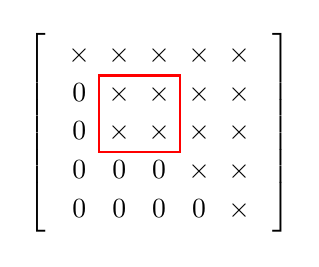
\begin{tikzpicture}
    \matrix[matrix of math nodes,
            nodes in empty cells,
            left delimiter={[},
            right delimiter={]}] (m) 
    {
        \times & \times & \times & \times & \times\\ 
        0      & \times & \times & \times & \times\\
        0      & \times      & \times & \times & \times\\ 
        0      & 0      & 0      & \times & \times\\ 
        0      & 0      & 0      & 0 & \times\\ 
    };

    \draw[red,thick] (m-2-2.north west) rectangle (m-3-3.south east);
\end{tikzpicture}
\end{center}

\subsubsection{Accounting for Jordan Blocks}
To handle Jordan blocks during eigenvalue computation:
\begin{itemize}
    \item Identify where the subdiagonal element is non zero.
    \item Consider the Jordan block as shown in the image, solve the obtained $2\times2$ matrix for its eigenvalues.
    \item The obtained complex conjugate roots are eigenvalues of the matrix
\end{itemize}

\section{Chosen Algorithm}
\begin{algorithm}[H]
\caption{Eigenvalue Calculation}
\begin{algorithmic}[1]
\REQUIRE A square matrix $A \in \mathbb{C}^{n \times n}$
\ENSURE Eigenvalues of $A$

\STATE To Upper Hessenberg form (via Householder reflection):
    \FOR{$k = 1$ TO $n-2$}
        \STATE Compute Householder reflector $P_k$ to zero out subdiagonal elements.
        \STATE Update $A$: $A \leftarrow P_k A P_k^T$
    \ENDFOR

\STATE QR Decomposition (via Givens Rotation):
\WHILE{not converged}
    \STATE QR Decomposition:
        \FOR{$k = 1$ TO $n-1$}
            \STATE Compute Givens rotation matrix $G_k$ to zero out the $(k+1, k)$ element.
            \STATE Apply $G_k$ from the left and right to $A$.
        \ENDFOR
    \STATE Form $A \leftarrow R Q$
\ENDWHILE
\STATE Extract Eigenvalues from Quasi-Triangular Matrix
\FOR{$i = 1$ TO $n$}
        \IF{$|A_{i+1, i}| < \epsilon$}
            \STATE Eigenvalue: $\lambda_i = A_{i, i}$
        \ELSE
            \STATE Compute eigenvalues of the $2 \times 2$ submatrix by solving quadratic:
            \begin{align*}
            \begin{bmatrix}
                A_{i, i} & A_{i, i+1} \\
                A_{i+1, i} & A_{i+1, i+1}
            \end{bmatrix}
            \end{align*}
        \ENDIF
    \ENDFOR
\RETURN Eigenvalues $\lambda_1, \lambda_2, ..., \lambda_n$
\end{algorithmic}
\end{algorithm}
The eigenvalue computation algorithm combines:
\begin{enumerate}
    \item \textbf{Householder Transformations:} To reduce the matrix to Hessenberg form, simplifying subsequent computations.
    \item \textbf{QR Iterations with Givens Rotations:} To iteratively compute an upper triangular matrix, where the diagonal elements converge to the eigenvalues.
\end{enumerate}

\section{Time Complexity Analysis}
\begin{enumerate}
\item{\textbf{Householder Transformations}}
Reducing an $(n \times n)$matrix to Hessenberg form takes $O(n^3)$ operations.

\item{\textbf{QR Iterations}}
Each QR decomposition requires $O(n^2)$ operations, on $n-1$ rows. Overall time complexity is $O(n^3)$ 

\item{\textbf{Overall Complexity}}
The total time complexity of the combined approach is $O(n^3)$, making it one of the better eigenvalue computation methods.
\end{enumerate}
\section{Comparison of Algorithms}

Effectiveness of eigenvalue algorithms is relative. Each algorithms have their own pros and cons. For instance, while an algorithm like Jacobi will work best, but it is limited to real, symmetric matrices. Below are a few popular algorithms, with their time complexities, pros, cons, conditions.

\begin{longtable}{|p{2.5cm}|p{3.5cm}|p{3.5cm}|p{2.5cm}|p{2.5cm}|}
\hline
\textbf{Algorithm} & \textbf{Pros} & \textbf{Cons} & \textbf{Time Complexity} & \textbf{Conditions} \\ \hline
\endfirsthead
\hline
\textbf{Algorithm} & \textbf{Pros} & \textbf{Cons} & \textbf{Time Complexity} & \textbf{Conditions} \\ \hline
\endhead
Householder + Givens & Stable, precise; preserves sparsity. & Complex preprocessing for Hessenberg form. & \( O(n^3) \) & Any square matrix. \\ \hline
Jacobi Method & Accurate for symmetric matrices; simple. & Slow for non-symmetric matrices; inefficient for large ones. & \( O(n^3) \) (dense) & Symmetric (real/complex). \\ \hline
Lanczos Algorithm & Efficient for sparse symmetric matrices. & Sensitive to rounding; limited to Hermitian matrices. & \( O(kn^2) \) & Sparse, symmetric/Hermitian. \\ \hline
QR Algorithm & Robust for eigenvalue computation. & High cost for large dense matrices. & \( O(n^3) \) & Any square matrix. \\ \hline
Arnoldi Algorithm & Handles non-symmetric sparse matrices. & Requires re-orthogonalization; less stable. & \( O(kn^2) \) & Sparse, any matrix. \\ \hline
Power Iteration & Simple, finds dominant eigenvalue. & Only computes the largest eigenvalue; slow for close eigenvalues. & \( O(kn^2) \) & Any square matrix. \\ \hline
\end{longtable}

\subsubsection*{Why Givens + Householder is Preferred}
\textbf{Householder Transformations:}
\begin{itemize}
    \item Efficient for reducing matrices to a simpler form (upper Hessenberg or tridiagonal).
    \item Provides numerical stability.
    \item Reduces the complexity of subsequent steps, like QR decomposition.
\end{itemize}
\textbf{Givens Rotations:}
\begin{itemize}
    \item Ideal for zeroing specific matrix elements without affecting others.
    \item Well-suited for sparse matrices.
    \item Simple to implement and numerically stable.
\end{itemize}
\textbf{Advantages:}
\begin{itemize}
\item This algorithm has no limitation in terms of what the enteries of the matrix can be (i.e. complex/real enteries), or on what the matrix has to be (ex: matrix does not have to be only symmetric/hermitian for it to work). 
\item The chosen algorithm of Givens rotations and Householder reflections balances numerical stability and efficiency. 
\item By reducing a matrix to Hessenberg form using Householder transformations and iteratively zeroing out elements with Givens rotations, it preserves orthogonality and sparsity while accelerating rate of convergence. 
\item Implementing a shift like Rayleigh quotient, rate of convergence drastically increases. 
\end{itemize}


\section{Conclusion}
The C-Code can be found at 
{\footnotesize
\begin{lstlisting}
https://github.com/ArjunPavanje/Matrix-Theory/tree/main/eigenvalues
\end{lstlisting}
}
\section{References}
\begin{thebibliography}{9}

\bibitem{youtube1} 
ETH Zurich \textit{QR Algorithms}. Available at: \url{https://people.inf.ethz.ch/arbenz/ewp/Lnotes/chapter4.pdf}.

\bibitem{youtube2} 
#Blue1Brown. \textit{Essence of Linear Algebra Playlist}. Available at: \url{https://youtube.com/playlist?list=PLZHQObOWTQDPD3MizzM2xVFitgF8hE_ab&si=oxNwAmrJMTRl0K5V}.

\bibitem{axler} 
Axler, S. (2024). \textit{Linear Algebra Done Right (4th ed.)}. Available at: \url{https://www.linear.axler.net/LADR4e.pdf}.

\bibitem{wiki} 
Wikipedia contributors. (2024). \textit{Eigenvalue algorithm}. Available at: \url{https://en.wikipedia.org/wiki/Eigenvalue_algorithm#Hessenberg_and_tridiagonal_matrices}.

\bibitem{Latex Template} 
    Latex. \textit{Latex Template}. Available at: \url{https://www.overleaf.com/latex/templates/uoe-report-dissertation-template/dnvsxhczdcpr}.
\end{thebibliography}
\end{document}



